\subsection{\texorpdfstring{\(p\) 次幂可积函数}{p 次幂可积函数}}

向量空间 \(\mathcal{K}(X;F)\) （若不致引起混淆，我们简记作 \(K_{F}\) ）由 X 到 F 中的具有紧支集的连续函数组成，它显然是每个向量空间 \(F_{F}^{p}\) 的子空间。

定义 2. --- 给定一个局部紧空间 X、X 上的一个测度 \(\mu\) 与一个 Banach 空间 F，我们用 \(\mathcal{L}_{\mathrm{F}}^{p}(\mathrm{X},\mu)\) （或简作 \(\mathcal{L}_{\mathrm{F}}^{p}(\mu)\) ，或 \(\mathcal{L}_{\mathrm{F}}^{p}\) ）表示局部凸空间 \(\mathcal{F}_{\mathrm{F}}^{p}(\mathrm{X},\mu)\) 中由 X 到 F 中的具有紧支集的连续映射所成的向量空间 \(\mathcal{K}(\mathrm{X};\mathrm{F})\) 的闭包。我们用 \(\mathrm{L}_{\mathrm{F}}^{p}(\mathrm{X},\mu)\) （或 \(\mathrm{L}_{\mathrm{F}}^{p}(\mu)\) ，或 \(\mathrm{L}_{\mathrm{F}}^{p}\) ）表示与 \(\mathcal{L}_{\mathrm{F}}^{p}(\mathrm{X},\mu)\) 相伴的（赋范）Hausdorff 空间。属于 \(\mathcal{L}_{\mathrm{F}}^{p}\) 的函数称为 \(p\) 次幂可积函数（*）。

显然 \(\mathcal{L}_{\mathrm{F}}^{p}(\mathrm{X},|\mu |) = \mathcal{L}_{\mathrm{F}}^{p}(\mathrm{X},\mu)\) 且 \(\mathrm{L}_{\mathrm{F}}^{p}(\mathrm{X},|\mu |) = \mathrm{L}_{\mathrm{F}}^{p}(\mathrm{X},\mu)\) 。

我们将用 \(L^{p}\) 与 \(L^{p}\) 代替 \(L_{R}^{p}\) 与 \(L_{R}^{p}\) （当这不致引起混淆时，或用 \(L_{C}^{p}\) 与 \(L_{C}^{p}\) 代替）。若 F 是一个复 Banach 空间，则 \(L_{F}^{p}\) 与 \(L_{F}^{p}\) 赋有域 C 上的拓扑向量空间结构（No.~3, 注）。

显然，\(F_{F}^{p}\) 中每个与 \(L_{F}^{p}\) 中一个函数等价的函数都属于 \(L_{F}^{p}\) 。取值于 F 且在 X 上几乎处处有定义的函数，若它与 \(L_{F}^{p}\) 中的一个函数等价，也称为 p 次幂可积的；类似地，取值于 \(\overline{R}\) 、在 X 上几乎处处有定义且有限的函数，若它与 \(L^{p}\) 中的一个函数等价，就称为 p 次幂可积的。

于是，\(L_{F}^{p}\) （相应地 \(L^{p}\) ）中的函数就是在整个 X 上有定义（相应地，在整个 X 上有定义且有限）的 p 次幂可积函数。在本节及下一节中，对 \(L_{F}^{p}\) （相应地 \(L^{p}\) ）中的函数证明的大多数命题，都可以立即推广到并非处处有定义（相应地，并非处处有定义且有限）的 p 次幂可积函数；我们通常把陈述并证明这些结果的任务留给读者。

注记. --- 1) 如已指出的（§2, No.~5），取值于 F 的 p 次幂可积函数一般不构成向量空间。

\begin{enumerate}
\def\labelenumi{\arabic{enumi})}
\setcounter{enumi}{1}
\tightlist
\item
  一般地，空间 \(\mathcal{F}_{\mathrm{F}}^{p}\) 不同于其子空间 \(\mathcal{L}_{\mathrm{F}}^{p}\) （§4, 习题 8）。
\end{enumerate}

定义 2 立即给出下述判别法：

命题 7. --- 为使函数 f 属于 \(L_{F}^{p}\) ，必须且只须对每个 \(\varepsilon > 0\) ，存在具有紧支集的连续函数 g 使 \(\mathrm{N}_{p}(\mathbf{f} - \mathbf{g}) \leqslant \varepsilon\) 。

换句话说，\(L_{F}^{p}\) 中的函数是具有紧支集的连续函数序列（对于 p 阶平均收敛拓扑）的极限。

命题 8. --- 设 f 是几乎处处有定义的数值函数（有限或非有限）；若对每个 \(\varepsilon > 0\) ，存在两个 p 次幂可积函数 g、h ，使 \(g \leqslant f \leqslant h\) 几乎处处成立且 \(\mathrm{N}_{p}(h - g) \leqslant \varepsilon\) ，则 f 是 p 次幂可积的。

因为，\(f\) 几乎处处有限且 \(\mathrm{N}_p(f - g) \leqslant \mathrm{N}_p(h - g) \leqslant \varepsilon\) ；于是命题 7 表明 \(f\) 是 \(p\) 次幂可积的。

由于按定义 \(L_{F}^{p}\) 是 \(F_{F}^{p}\) 的一个闭子空间，且后一空间是完备的（No.~3, 命题 5），我们有下述结果（GT, II, §3, No.~4, 命题 8）：

定理 2. --- 空间 \(\mathcal{L}_{\mathrm{F}}^{p}\) 是完备的；空间 \(\mathrm{L}_{\mathrm{F}}^{p}\) 是一个 Banach 空间。

在空间 \(L_{F}^{p}\) 中，一个类的范数 \(\mathrm{N}_{p}(\widetilde{\mathbf{f}})\) 也记作 \(\| \widetilde{f} \|_{p}\) 。

定理 2 可以加强如下：

定理 3. --- 设 \((\mathbf{f}_n)\) 是空间 \(\mathcal{L}_{\mathrm{F}}^p\) 中的一个 Cauchy 序列；存在一个子序列 \((\mathbf{f}_{n_k})\) （\((\mathbf{f}_n)\) 的），它具有下列性质：

\(1^{\circ}\) 通项为 \(\mathrm{N}_p(\mathbf{f}_{n_{k + 1}} - \mathbf{f}_{n_k})\) 的级数收敛；

\(2^{\circ}\) 通项为 \(\mathbf{f}_{n_{k+1}}(x) - \mathbf{f}_{n_k}(x)\) 的级数几乎处处绝对收敛；

\(3^{\circ}\) 若 \(\mathbf{f}\) 是定义在 X 上且几乎处处等于序列 \((\mathbf{f}_{n_k}(x))\) 的极限的函数，则 \(\mathbf{f}\) 属于 \(\mathcal{L}_{\mathrm{F}}^p\) 且序列 \((\mathbf{f}_n)\) \(p\) 阶平均收敛于 \(\mathbf{f}\) ；

\(4^{\circ}\) 存在下半连续函数 \(g \geqslant 0\) 使 \(\mathrm{N}_p(g) < +\infty\) ，且对每个 \(k\) ，有 \(|\mathbf{f}_{n_k}(x)| \leqslant g(x)\) 对所有 \(x \in X\) 成立。

如同 No.~3 命题 5 的证明中那样，只需用归纳法定义序列 \((n_k)\) ，使 \(\mathrm{N}_p(\mathbf{f}_{n_{k+1}} - \mathbf{f}_{n_k}) \leqslant 2^{-k}\) ；于是 \(2^\circ\) 与 \(3^\circ\) 由 No.~3 的命题 6 以及 \(\mathcal{L}_{\mathrm{F}}^p\) 在 \(\mathcal{F}_{\mathrm{F}}^p\) 中为闭这一事实得出。另一方面，若 \(h(x)\) 是通项为 \(|\mathbf{f}_{n_{k+1}}(x) - \mathbf{f}_{n_k}(x)|\) 的级数的和，则 No.~2 的定理 1 表明 \(\mathrm{N}_p(h) < +\infty\) ；因此，由 \(|\mu|^*\) 的定义，存在下半连续函数 \(g \geqslant h + |\mathbf{f}_{n_1}|\) 使 \(\mathrm{N}_p(g) < +\infty\) ，证明遂告完成。

推论 1. --- 若 Cauchy 序列 \((\mathbf{f}_{n})\) （空间 \(L_{F}^{p}\) 中的）使序列 \((\mathbf{f}_{n}(x))\) 几乎处处收敛于 \(\mathbf{f}(x)\) ，则 f 是 p 次幂可积的，且序列 \((\mathbf{f}_{n})\) p 阶平均收敛于 f。

因为，存在子序列 \((\mathbf{f}_{n_{k}})\) （\((\mathbf{f}_{n})\) 的），使 \((\mathbf{f}_{n_{k}}(x))\) 几乎处处收敛于 \(\mathbf{g}(x)\) ，其中 g 是 \(L_{F}^{p}\) 中的一个函数，使 \((\mathbf{f}_{n})\) p 阶平均收敛于 g。于是假设蕴涵 \(\mathbf{f}(x)=\mathbf{g}(x)\) 几乎处处成立，推论得证。

推论 2. --- 设 E 是 \(L_{F}^{p}\) 的一个稠密子集。对每个函数 \(f \in L_{F}^{p}\) ，存在 E 中函数的一个序列 \((\mathbf{g}_{n})\) ，它具有下列性质：

\(1^{\circ}\) 序列 \((\mathbf{g}_n)\) \(p\) 阶平均收敛于 \(\mathbf{f}\) ；

\(2^{\circ}\) 对几乎每个 \(x \in \mathbf{X}\) ，序列 \((\mathbf{g}_n(x))\) 收敛于 \(\mathbf{f}(x)\) 。

因为，由于空间 \(L_{F}^{p}\) 是可度量的，存在一个 Cauchy 序列 \((\mathbf{f}_{n})\) （\(L_{F}^{p}\) 中的），由 E 中的函数组成且 p 阶平均收敛于 f（GT, IX, §2, No.~6, 命题 8）；只需对这个序列应用定理 3。

推论 2 特别适用于取 E 为具有紧支集的连续函数所成的空间 \(K_{F}\) 的情形。

\pandocbounded{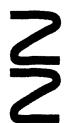
\includegraphics[keepaspectratio]{images/part001_fce77adb.jpg}}

注记. --- 1) Cauchy 序列 \((\mathbf{f}_n)\) （\(\mathcal{L}_{\mathrm{F}}^{p}\) 中的）可以使序列 \((\mathbf{f}_n(x))\) 在 X 的任何点都不收敛（习题 1）。

\begin{enumerate}
\def\labelenumi{\arabic{enumi})}
\setcounter{enumi}{1}
\tightlist
\item
  若 \(\mathbf{f}\) 属于 \(\mathcal{L}_{\mathrm{F}}^{p}\) ，并不总能找到具有紧支集的连续函数的序列 \((\mathbf{f}_n)\) ，使序列 \((\mathbf{f}_n(x))\) 在 \(X\) 上处处收敛于一个几乎处处等于 \(\mathbf{f}(x)\) 的函数（§4, 习题 4 c)）。
\end{enumerate}

